
\documentclass[conference]{IEEEtran}

%% Language and font encodings
\usepackage[english]{babel}
\usepackage[utf8x]{inputenc}
\usepackage[T1]{fontenc}

%% Sets page size and margins
\usepackage[a4paper,top=2cm,bottom=3cm,left=2cm,right=2cm,marginparwidth=1.75cm]{geometry}

%% Useful packages
\usepackage{amsmath}
\usepackage{graphicx}
\usepackage[colorinlistoftodos]{todonotes}
\usepackage[colorlinks=true, allcolors=blue]{hyperref}
\usepackage{graphicx}
\usepackage{amssymb}
\usepackage{lineno}
\usepackage{float}
\usepackage{caption}
\usepackage{subcaption}


\IEEEoverridecommandlockouts
\usepackage{cite}
\usepackage{amsmath,amssymb,amsfonts}
\usepackage{algorithmic}
\usepackage{textcomp}
\usepackage{xcolor}
\usepackage{textgreek}
\usepackage{rotating}
\usepackage{multirow}
\usepackage{multicol}
\graphicspath{ {images/} }

\begin{document}

\title{Model Based Predictive Control for a Smart Conveyor Belt System}

\author{\IEEEauthorblockN{David Reixach-Pérez}
\IEEEauthorblockA{
\textit{Master Degree in Automatic Control and Robotics} \\
\textit{ETSEIB - Universitat Politècnica de Catalunya, Barcelonatech} \\
\textit{david.reixach@estudiant.upc.edu}
}
}

\maketitle

\begin{abstract}
This paper proposes a MPC solution for a logistic system modeled as a 2-DOF manipulator. A formulation and a non-linear model is derived. A linearized approach for this model is stated. A multilayer control architecture is considered. LMPC and NMPC are considered for solving such problem, formulating the corresponding OCPs. Simulation for both propositions is performed and results are presented and discussed. Some conclusions are given regarding the work done.
\end{abstract}

\begin{IEEEkeywords}
Model Predictive Control; LMPC; NMPC; Multilayer Control Architecture; Kinematic Model; Dynamic Model; Simulation;
\end{IEEEkeywords}

\section{Introduction}

Recent development in robotics and control science provide new possibilities for handling classical logistic problems. In this work we propose a control solution for a smart conveyor belt for packages. The smart conveyor belt is a discretized finite surface for which linear velocity -magnitude and direction- can be set at each point independently. Understood as a roller conveyor, the velocity is transmitted to the package by means of friction. Each point represent a roller, for which rotating speed and orientation on the surface can be controlled.

We understand the control problem as a multilayer case. First, the package is modeled as a two-degree-of-freedom robot. A model based controller obtains a desired linear and angular velocity for its point within the surface, what with the use of the conveyor inverse kinematics model produces the desired linear velocity for each discretized point, that can be easily translated to rotating speed and angular position. Then a second control layer would ensure the actuators following its reference, for example independent PID controllers for each actuator.

Developing a dynamic model for our manipulator would be a task of a high complexity. We would have to include the dynamic behavior of the actuators and build a model that would depend on the position of the package as forces are only transmitted along its contact surface. However, a simplest yet powerful approach could be to embed actuators effect on the package as a dragging force and torque. This could provide a richer controller (e.g. friction force limitations). In this case study but, we exclusively relay on the kinematic model for the system as our scope is to follow a given trajectory minimizing tracking error and control effort.

Our objective is to implement a Model Predictive Control. In order to achieve fast convergence for the Optimal Control Problem (OCP) we first consider a linearized model and we propose a Linear MPC (LMPC). Also, due to its Non-linear nature we will consider a Non-linear MPC (NMPC) and will proceed with a fair comparison between methods. The document is structured as follows, in Section II the mathematical model is presented, in Section III the design of the control problem is stated, in Section IV experimentation and results are explained and in Section V conclusions are given.

\section{Problem Formulation}

In Fig. \ref{fig:problem} a representation of our problem is shown. The formulation is split between two models, the kinematic model of the box understood as a 2-Degree-of-Freedom robot controlled by its linear and angular velocity; and the inverse kinematics model of the surface, in order to compute the velocity vector field needed to produce the desired control effect to the box.

The first model will be used to generate a MPC controller that ensures tracking a reference (position and orientation) and the second one to generate the desired reference trajectories to the actuators.

\begin{figure}[H]
\centering
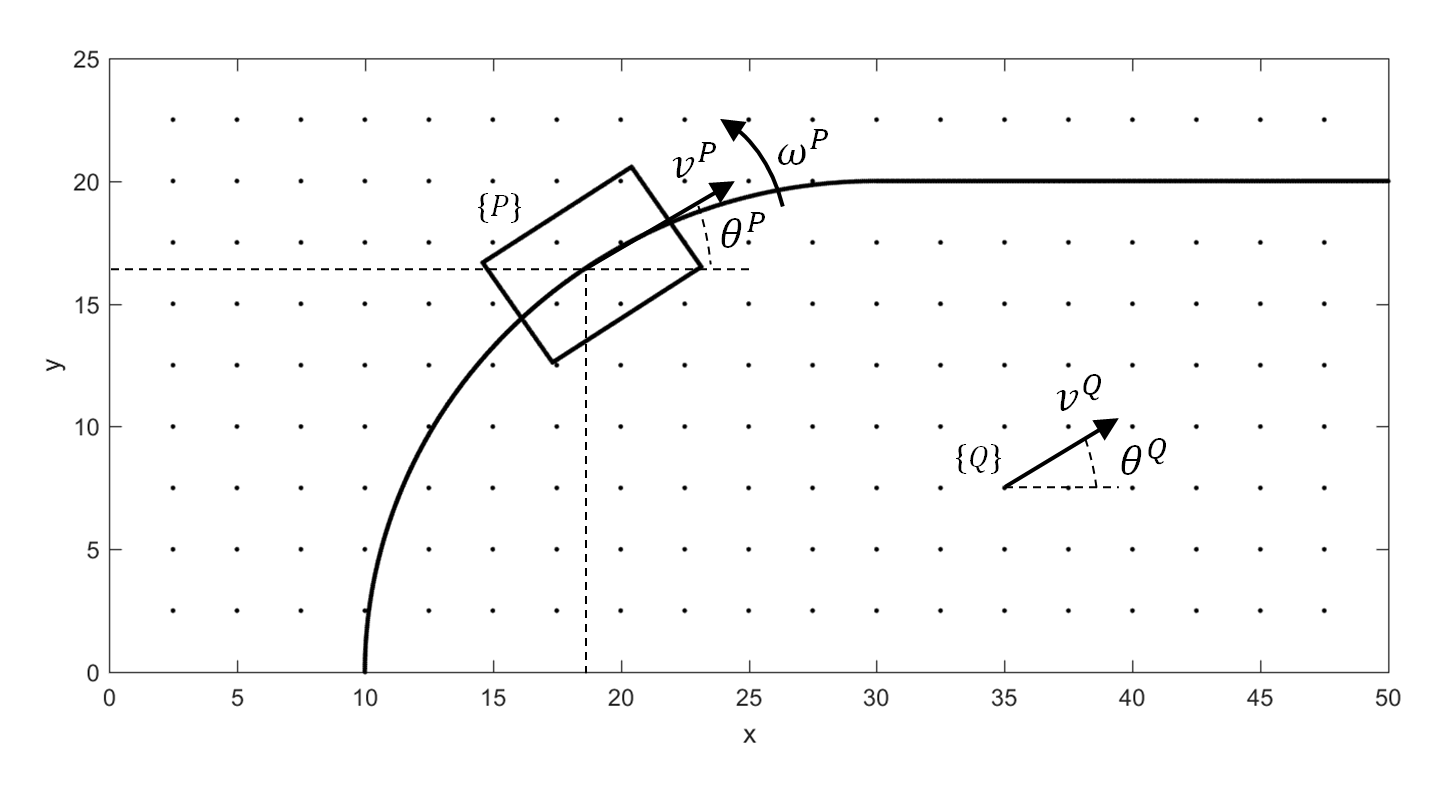
\includegraphics[width=0.5\textwidth]{problem_variables.PNG}
\caption{\label{fig:problem}Problem formulation. P refers to box variables (top layer states and control actions) and Q to actuators state.}
\end{figure}

\subsection{Non-linear model}\label{AA}

The kinematic model for the package simplified as a 2-DOF robot, according to \cite{campion1996structural} is given by:

\begin{equation} \label{eq:1}
\dot{X} =  \left[\begin{array}{c}
\dot{x} \\ \dot{y} \\ \dot{\theta} \end{array}\right]
 = \left[\begin{array}{c}
v(t)cos(\theta(t)) \\ v(t)sin(\theta(t)) \\ \omega(t) \end{array}\right]
\end{equation}

And it can be easily discretized:

\begin{equation} \label{eq:2}
\left[\begin{array}{c}
x(k+1) \\ y(k+1) \\ \theta(k+1) \end{array}\right]
 = \left[\begin{array}{c}
x(k)+v(k)T_{s}cos(\theta(k)) \\ y(k)+v(k)T_{s}sin(\theta(k)) \\ \theta(k)+T_{s}\omega(k) \end{array}\right]
\end{equation}

Our Non-linear discrete-time approach assumes model time-invariance at each step, the full state is measured and no presence of disturbances.

\subsection{Linear model}\label{AB}

The kinematic model previously obtained can be linearized at instant (k), giving to the next expression:

\begin{equation} \label{eq:3}
\tilde{x}(k+1)=\mathbf{A}(k)\tilde{x}(k)+\mathbf{B}(k)\tilde{u}(k)
\end{equation}

with

\begin{equation*} 
\mathbf{A}(k) \triangleq
\left[\begin{array}{ccc}
1 & 0 & -v(k)T_{s}sin(\theta(k)) \\
0 & 1 & v(k)T_{s}cos(\theta(k)) \\ 
0 & 0 & 1 \end{array}\right]
\end{equation*}

\begin{equation*} 
\mathbf{B}(k) \triangleq
\left[\begin{array}{cc}
T_{s}cos(\theta(k)) & 0 \\
T_{s}sin(\theta(k)) & 0  \\ 
0 & T_{s} \end{array}\right]
\end{equation*}

\begin{equation*}
\tilde{x} \triangleq x-x_{k}
\end{equation*}

\begin{equation*} 
\tilde{u} \triangleq u-u_{k}
\end{equation*}

Also, over the assumptions taken  for the previous model, a linear behavior is assumed, what is a valid approximation close to the linearizing point, but not much further away.

\subsection{Inverse Kinematics}\label{AC}

Understanding the kinematics of the 2-DOF robot as the composition of its linear and angular velocity and mapping them through its ICR, the velocity vector for a point Q can be obtained with respect to the velocity of P and their relative position:

\begin{equation} \label{eq:4}
(v_{x}^{Q},v_{y}^{Q})=(v_{x}^{P},v_{y}^{P})+(P_{y}-Q_{y},-P_{x}+Q_{x})\cdotp\dot{\theta}^{P}
\end{equation}

\section{Controllers design}

The MPC algorithm idea is to obtain the control input that plugged to a modeled system generates an optimum behavior along a sequence, according to a given law. The MPC computes at each sampling time the optimal control sequence for a prediction horizon ($H_{p}$), the first control signal is applied to the plant and the control loop is repeated again, shifting the prediction horizon accordingly. In Fig. \ref{fig:control} an application of the algorithm specific to our case can be seen.

In the next subsections we present the formulation of the OCP, for the LMPC and the NMPC.

\begin{figure}[H]
\centering
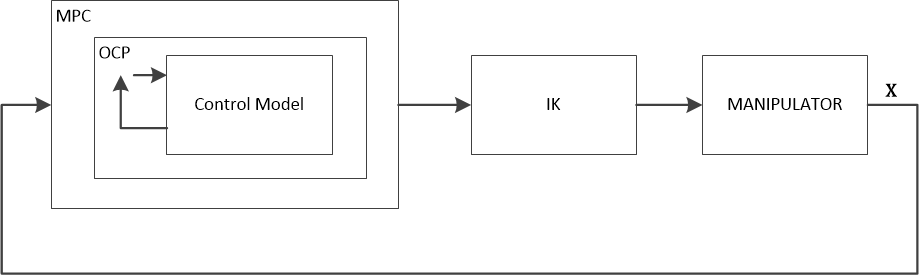
\includegraphics[width=0.5\textwidth]{control_loop.png}
\caption{\label{fig:control}Schema of the top control layer (MPC and Inverse Kinematics module). A bottom layer is considered embedded inside our plant block.}
\end{figure}

\subsection{LMPC}\label{BA}

The OCP for the LMPC simulation comes from the linearized model we obtained in the previous section. The optimization law is a weighted minimization of the 2-norm of both the error of the states w.r.t. the reference and the control action.

Eq. \ref{eq:5} defines the optimization function, the dynamic model together with the control limitations constraint the problem. As it is seen, for each prediction horizon, the dynamic model is linearized at the last obtained point (from the previous iteration), ($x_{r},u_{r}$), which do not correspond to the initial states for the current optimization.

\begin{equation} \label{eq:5}
\min_{\tilde{U}(k)}\left(\sum_{k=1}^{H_{p}}\tilde{e}(k)^{T}Q \tilde{e}(k)+
\sum_{k=0}^{H_{p}-1}\tilde{u}(k)^{T}R\tilde{u}(k)\right)
\end{equation}

s.t.

\begin{equation*}
\tilde{x}(k+1) = \mathbf{A}_{r}\tilde{x}(k)+\mathbf{B}_{r}\tilde{u}(k) \qquad \forall k \in [0,Hp]
\end{equation*}
\begin{equation*}
\mathbf{G}\tilde{u}(k) \leq \mathbf{b} \qquad \forall k \in [0,Hp]
\end{equation*}
\begin{equation*}
\tilde{x}(k) \in \Re^{3} \qquad \forall k \in [0,Hp]
\end{equation*}
\begin{equation*}
\tilde{u}(k) \in \Re^{2} \qquad \forall k \in [0,Hp]
\end{equation*}

with

\begin{equation*}
\mathbf{G} = \left[\begin{array}{cc} 1 & 0\\
0 & 1 \\
-1 & 0\\
0 & -1 \end{array}\right]
\end{equation*}
\begin{equation*}
\mathbf{b} = \left[\begin{array}{c} \overline{v} \\
\overline{\omega} \\
-\overline{v}\\
-\overline{\omega} \end{array}\right]
\end{equation*}
\begin{equation*}
\tilde{U}(k) \triangleq \left\lbrace \tilde{u}(k),\tilde{u}(k+1),...,\tilde{u}(k+H_{p}-1)\right\rbrace
\end{equation*}
\begin{equation*}
\tilde{e}(k) \triangleq \tilde{x}_{R}(k)-\tilde{x}(k)
\end{equation*}
\begin{equation*}
\tilde{x}(k) \triangleq x(k)-x_{r}
\end{equation*}
\begin{equation*}
\tilde{x}_{R}(k) \triangleq x_{R}(k)-x_{r}
\end{equation*}
\begin{equation*}
\tilde{u}(k) \triangleq u(k)-u_{r}
\end{equation*}

After some testing we obtain the matrices we use as weighting factors:

\begin{equation*}
Q = \left[\begin{array}{ccc} 10^3 & 0 & 0 \\
0 & 10^3 & 0 \\
0 & 0 & 10^3 \end{array} \right]
\end{equation*}
\begin{equation*}
R = \left[\begin{array}{cc} 0.1 & 0 \\
0 & 10^{-3} \end{array} \right]
\end{equation*}


\subsection{NMPC}\label{BB}

The OCP for the NMPC simulation comes directly from Eq. \ref{eq:1} as the problem is formulated in continuous time. The optimization law, in this case formulated in continuous time (integral), is the same as the LMPC OCP. Its complete formulation is proposed below:

\begin{equation} \label{eq:6}
\min_{u(t),t \in [0,T_{p}]}\int_{0}^{T_{p}}(e(t)^{T}Q e(t)+
u(t)^{T}Ru(t))dt
\end{equation}

s.t.

\begin{equation*}
\dot{X} = \left[\begin{array}{c}
v(t)cos(\theta(t)) \\ v(t)sin(\theta(t)) \\ \omega(t) \end{array}\right]
\end{equation*}
\begin{equation*}
\mathbf{G}u(t) \leq \mathbf{b} \qquad \forall t \in [0,Tp]
\end{equation*}
\begin{equation*}
X(t) \in \Re^{3} \qquad \forall t \in [0,Tp]
\end{equation*}
\begin{equation*}
u(t) \in \Re^{2} \qquad \forall t \in [0,Tp]
\end{equation*}

with:

\begin{equation*}
X(t) \triangleq \left[\begin{array}{ccc}
x(t) & y(t) & \theta(t) \end{array}\right]^{T}
\end{equation*}
\begin{equation*}
u(t) \triangleq \left[\begin{array}{cc}
v(t) & \omega(t)\end{array}\right]^{T}
\end{equation*}
\begin{equation*}
e(t) \triangleq X_{R}(t)-X(t)
\end{equation*}


weighting factors (also after some testing):

\begin{equation*}
Q = \left[\begin{array}{ccc} 100 & 0 & 0 \\
0 & 100 & 0 \\
0 & 0 & 80 \end{array} \right]
\end{equation*}
\begin{equation*}
R = \left[\begin{array}{cc} 1 & 0 \\
0 & 1 \end{array} \right]
\end{equation*}


\section{Simulation Results}

\subsection{Experiment design}\label{CA}
We develop a framework in MATLAB\textregistered{} for both experiments (LMPC and NMPC). In the first case, the MPC simulation is build making use of Yalmip Toolbox \cite{1393890}. In the second case we use ACADO Toolkit \cite{Houska2011a}. In both experiments we simulate the system with the non-linear model.

The design of the experiment includes a reference trajectory to follow and the definition of the initial states. In Fig. \ref{fig:problem} the reference trajectory for the linear position is seen. The angular position is defined as the tangent along the curve (the system has only 2-DOF). The trajectory is discretized in 800 points, what according to the sampling time chosen, $T_{s}$, is expected to be covered in 40s. The initial conditions for the states are assigned to the initial reference point, the initial conditions for the control actions are set to 0.

At the simulation stage, we include a low disturbance modeled as a noise. See the reformulation of the model below and other simulation parameters in Table \ref{tab:param}.

\begin{equation} \label{eq:6}
X(k+1) = f_{m}(X(k),u(k)) + \mathbf{E} w
\end{equation}

where $f_{m}$ corresponds to the simulation model, and with:

\begin{equation*}
\mathbf{E} = \left[\begin{array}{c}
1 \\ 1 \\ 0.1 \end{array}\right]
\end{equation*}
\begin{equation*}
w \sim \mathcal{N}(0,\sigma_{W}^2)
\end{equation*}

\begin{table}
\centering
\begin{tabular}{c|c|c|c}
	Name & Parameter & Value \\\hline
	Sample time & $T_{s}$ & 0.05 s \\
	Disturbance variance & $\sigma_{W}^2$ & 0.0011  \\
    Prediction horizon & $H_{p}$ & 5 \\
    $v$ bound & $\overline{v}$ & 10 u/s\\
    $\omega$ bound & $\overline{\omega}$ & 4 rad/s \\
\end{tabular}
\caption{\label{tab:param}Simulation and Model Parameters}
\end{table}

\subsection{Results for the LMPC}\label{CB}

Fig. \ref{fig:lmpc_simulation}. Show the simulation results for the LMPC. Regarding the error for the states, we mainly see an accumulation of the error for the \(y\) state. State \(x\) follows reliably the reference and state \(\theta\) results in a chattering behavior, probably is the most affected state by the perturbation, with increasing displacement interval but approximately following its reference trajectory.

Regarding the control actions, in both signals high chattering is observed, \(v\) gets often saturated, while \(\omega\) remains into the bounds.

\begin{figure}
\centering
\begin{subfigure}[t]{0.4\textwidth}
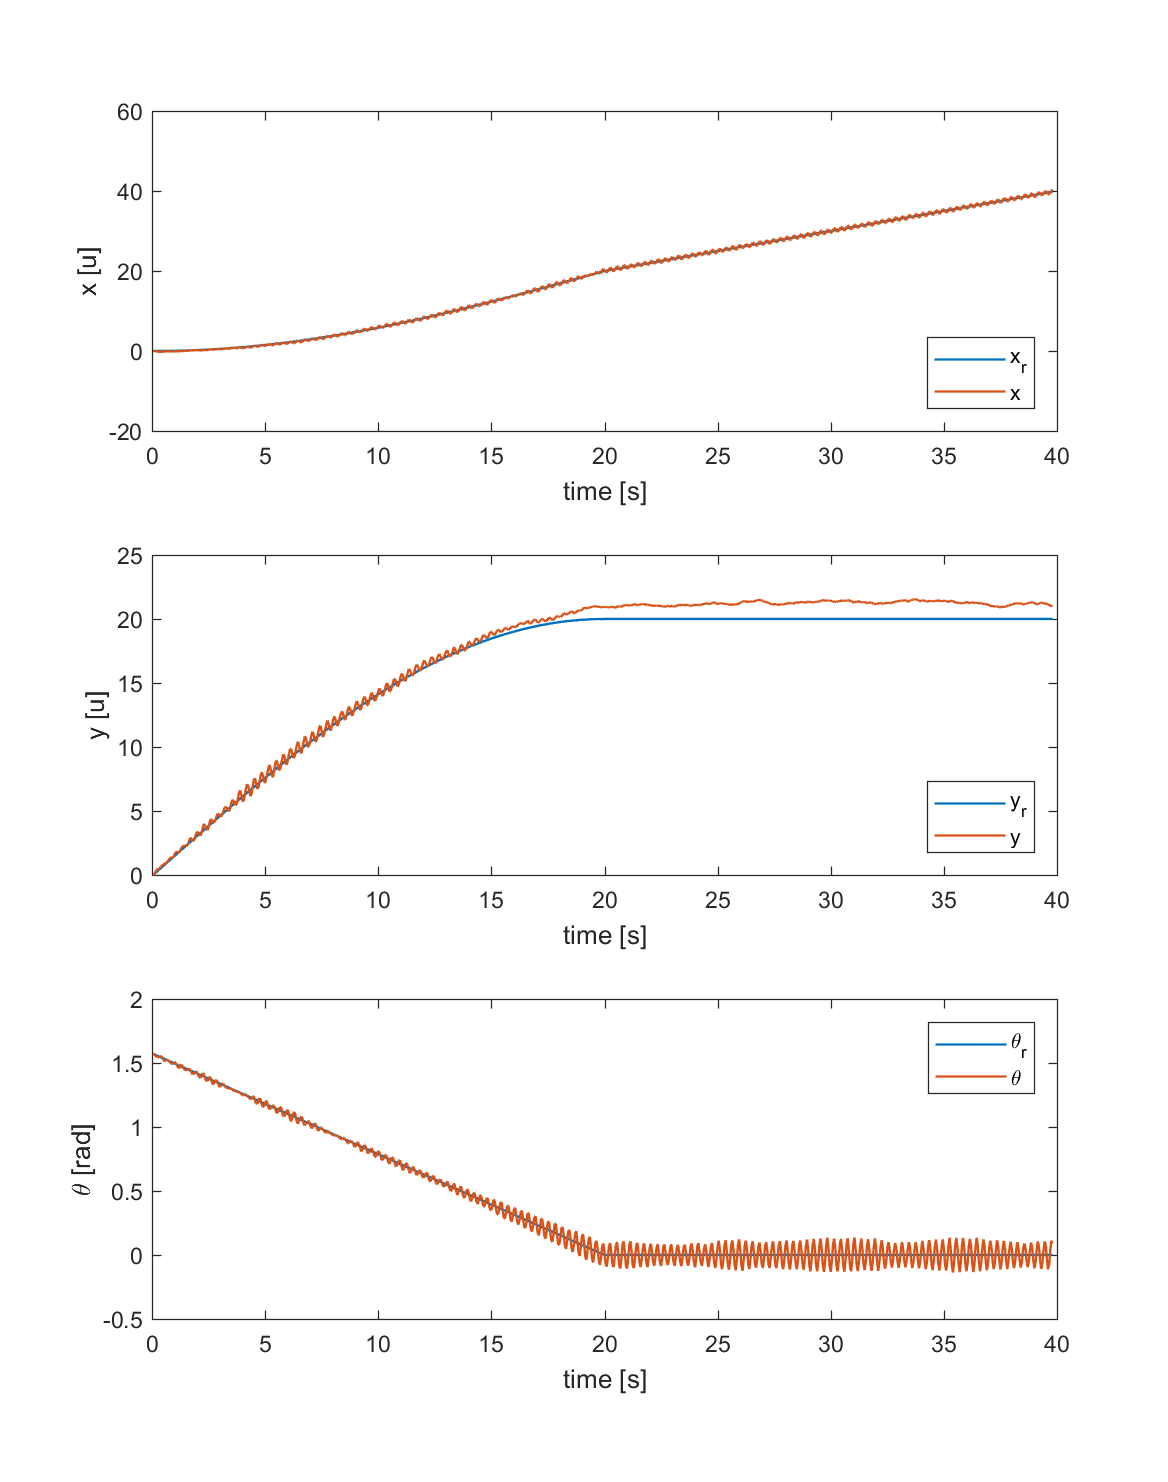
\includegraphics[width=1.2\textwidth]{lmpc_states.png}
\caption{\label{fig:lmpcxl}System's state behavior compared to its reference.}
\end{subfigure}
\begin{subfigure}[t]{0.4\textwidth}
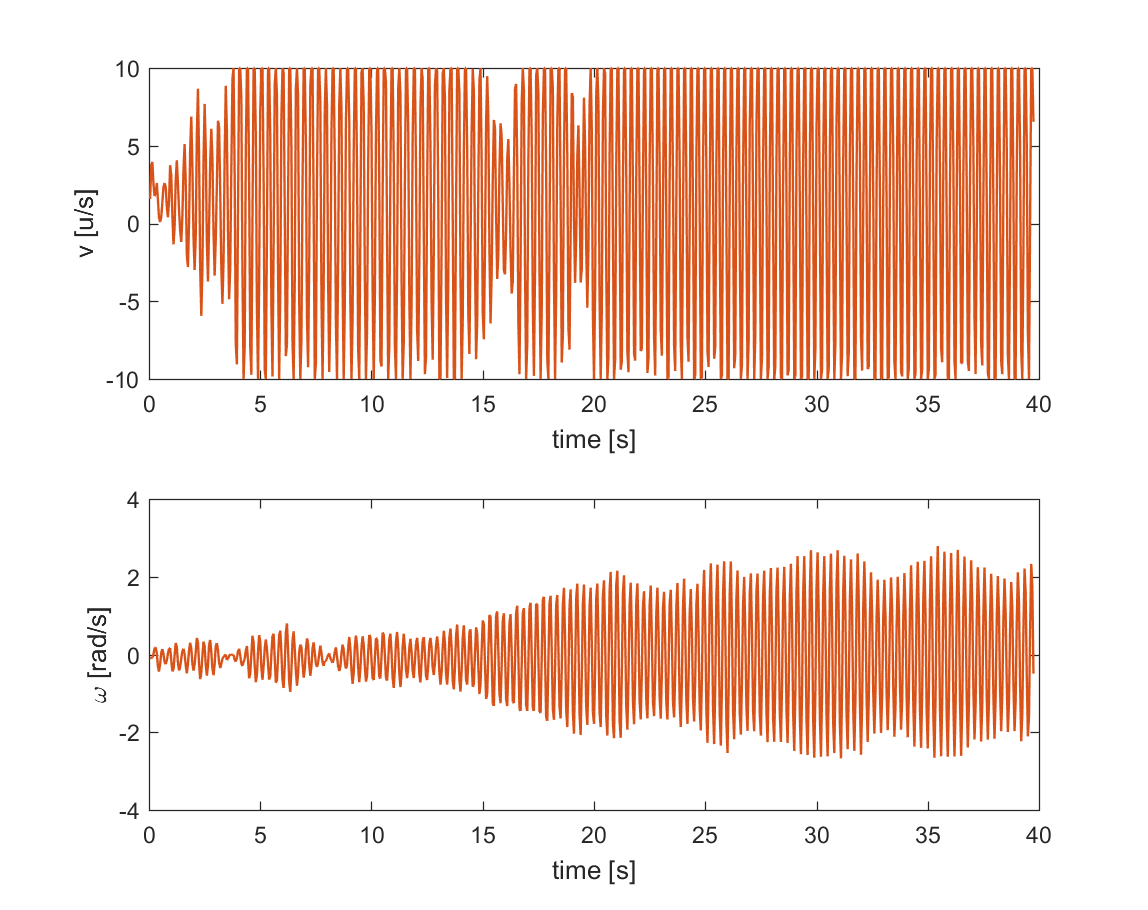
\includegraphics[width=1.2\textwidth]{lmpc_control.png}
\caption{\label{fig:lmpcu}Control action evolution.}
\end{subfigure}
\begin{subfigure}[t]{0.4\textwidth}
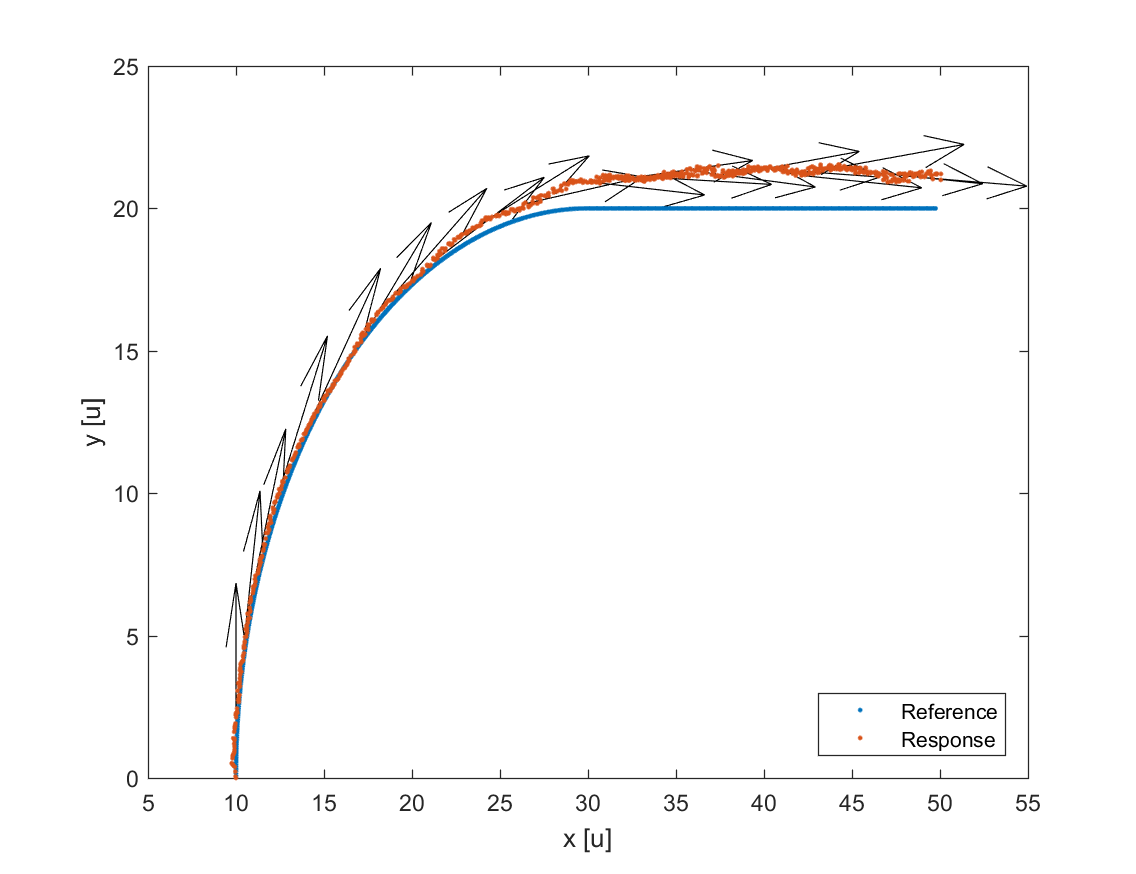
\includegraphics[width=1.2\textwidth]{lmpc_xy.png}
\caption{\label{fig:lmpcxy}Overall response of the system over the surface. Arrows at the given points correspond to orientation.}
\end{subfigure}
\caption{\label{fig:lmpc_simulation}LMPC Simulation: Compound of the obtained responses.}
\end{figure}

% \begin{figure}[H]
% \centering
% 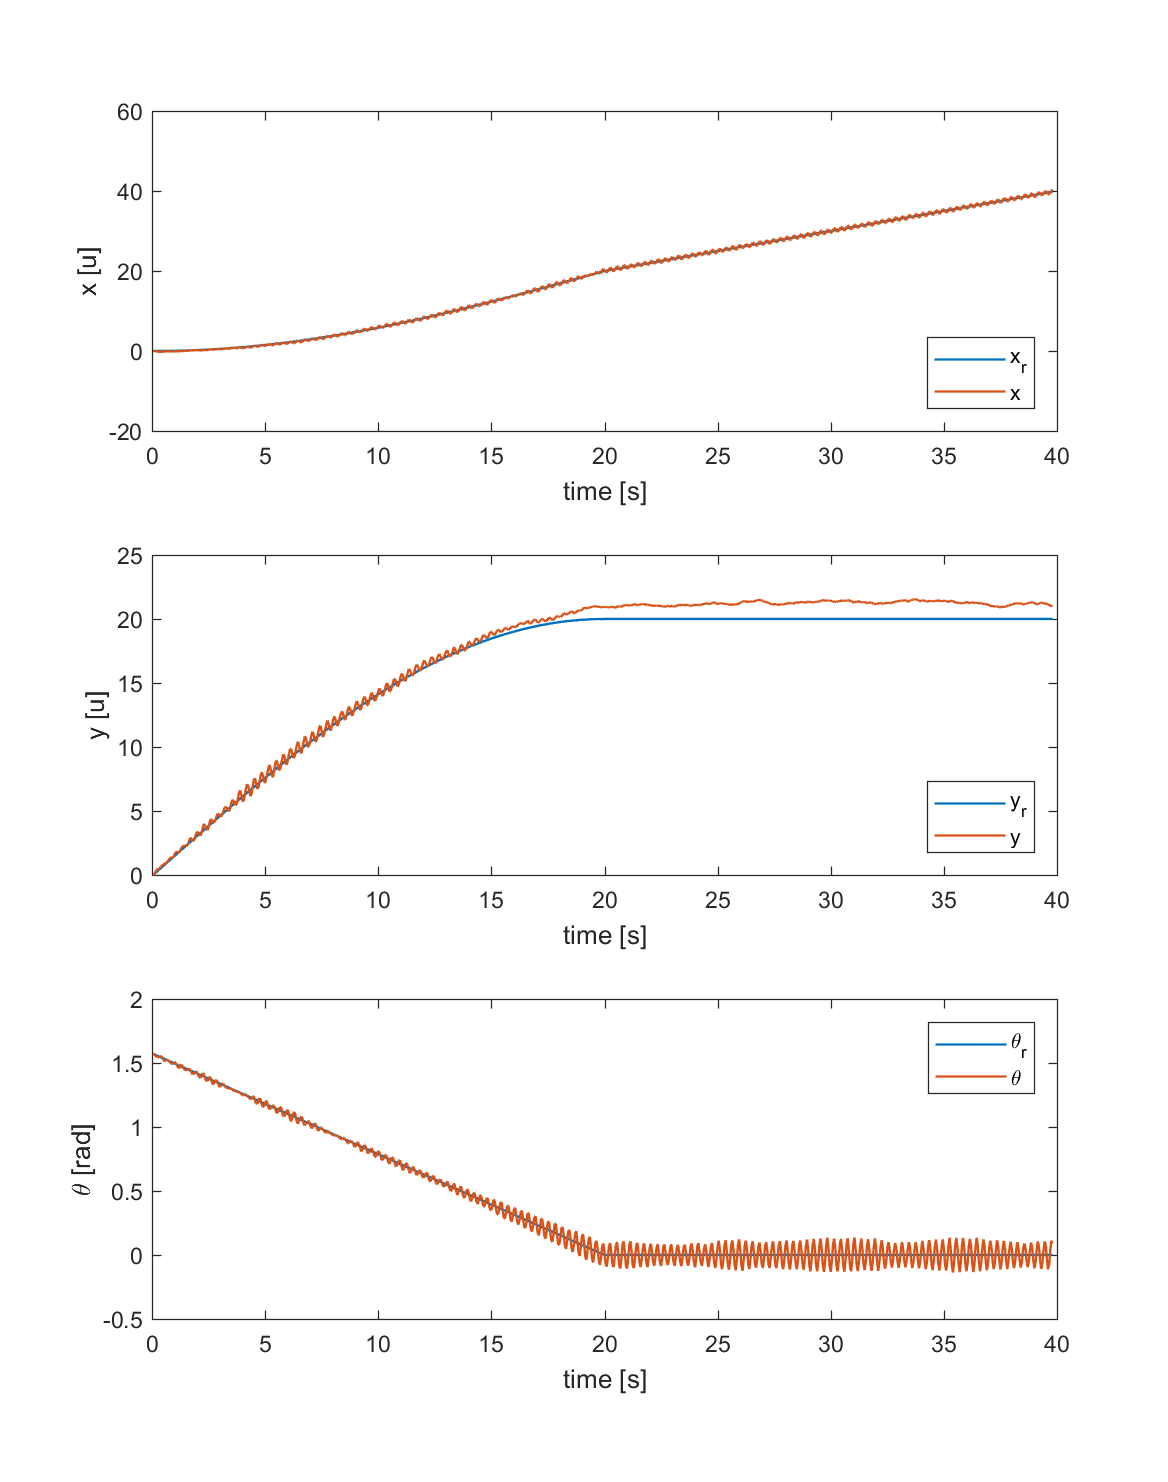
\includegraphics[width=0.5\textwidth]{lmpc_states.png}
% \caption{\label{fig:lmpcxl}LMPC Simulation: System's state behavior compared to its reference.}
% \end{figure}
% \begin{figure}[H]
% \centering
% 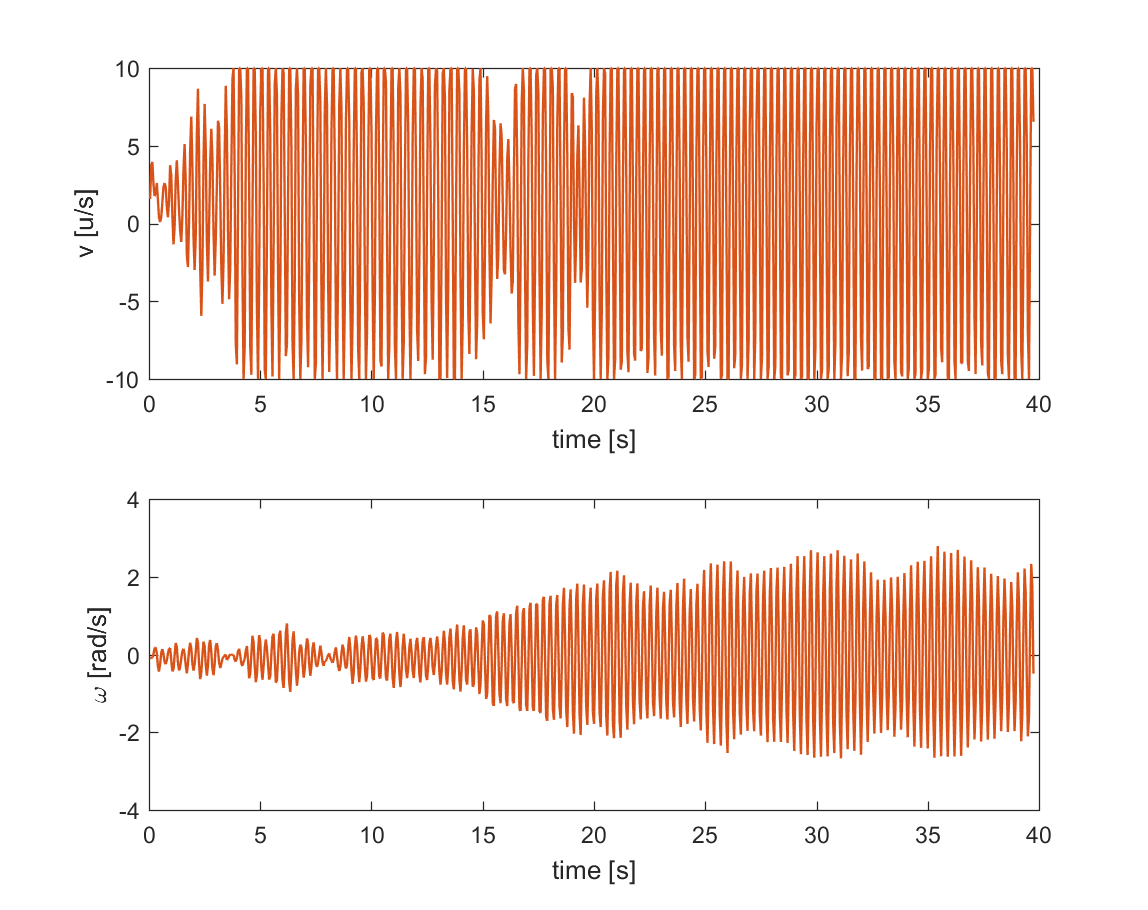
\includegraphics[width=0.5\textwidth]{lmpc_control.png}
% \caption{\label{fig:lmpcu}LMPC Simulation: Control action evolution.}
% \end{figure}
% \begin{figure}[H]
% \centering
% 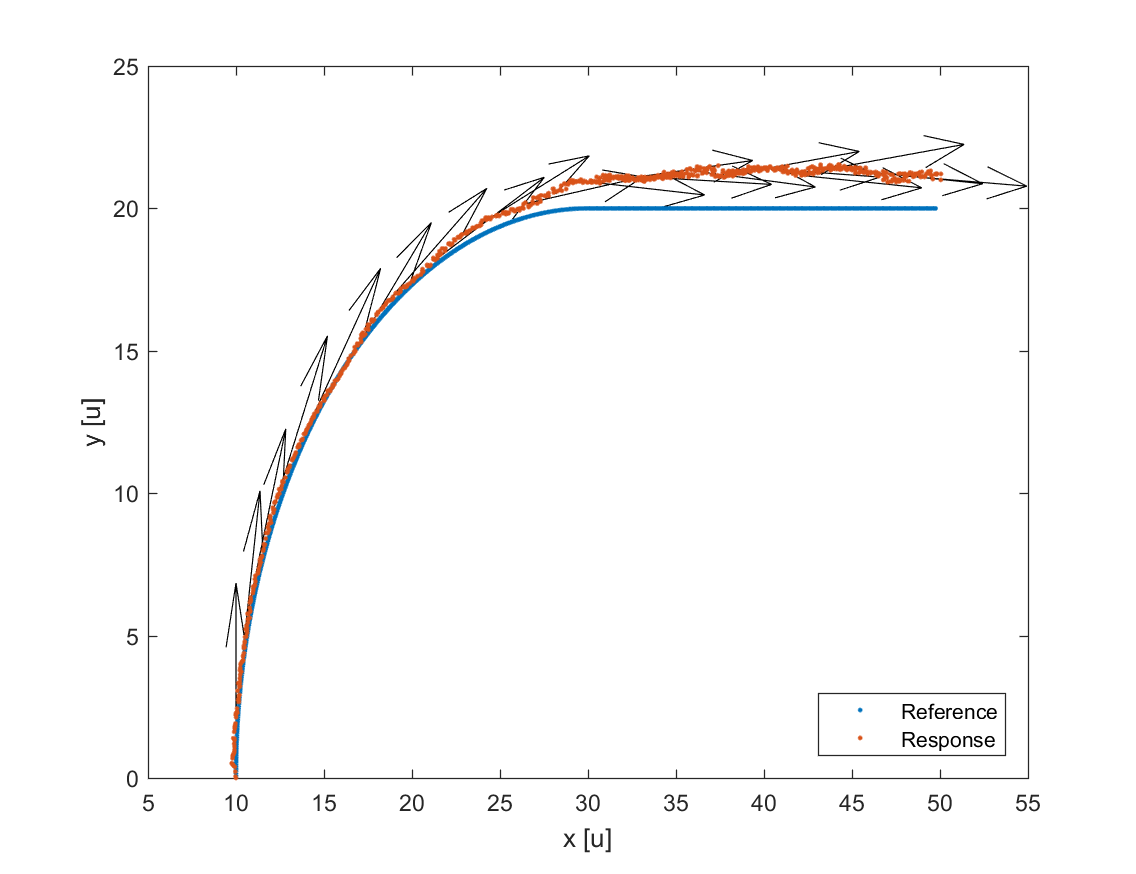
\includegraphics[width=0.5\textwidth]{lmpc_xy.png}
% \caption{\label{fig:lmpcxy}LMPC Simulation: Overall response of the system over the surface. Arrows at the given points correspond to orientation.}
% \end{figure}


\subsection{Results for the NMPC
\protect\footnote{\color{red}Due to a programming error, the presented results for the NPMC Simulation do not include the defined perturbation.\color{black}}}
\label{CC}

Fig. \ref{fig:nmpc_simulation}. Show the simulation results for the NMPC. Regarding the error for the states, despite a bit chattering, position states \((x,y)\) show a good tracking of the reference. State \(\theta\) shows a highly oscillating behavior, misleading.

Regarding the control actions, in both signals they show a clear oscillating behavior, despite their frequency is much lower than in the linear case. \(v\) remains into the bounds, while \(\omega\) gets closer to them, in some cases, saturation appears.

\begin{figure}
\centering
\begin{subfigure}[t]{0.4\textwidth}
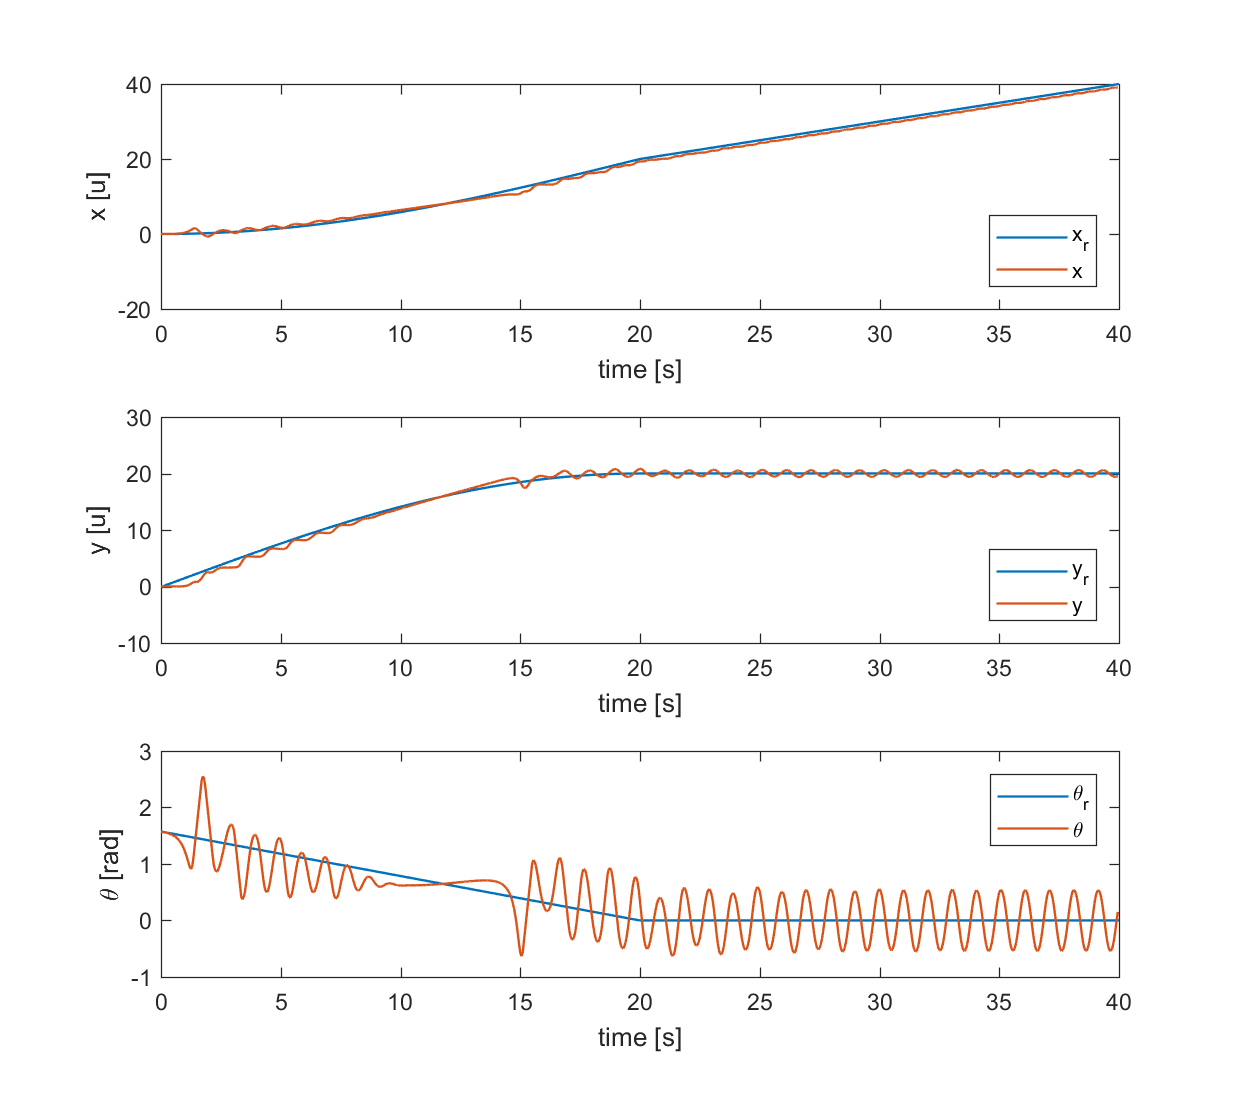
\includegraphics[width=1.4\textwidth]{nmpc_states.png}
\caption{\label{fig:nmpcxl}System's state behavior compared to its reference.}
\end{subfigure}
\begin{subfigure}[t]{0.4\textwidth}
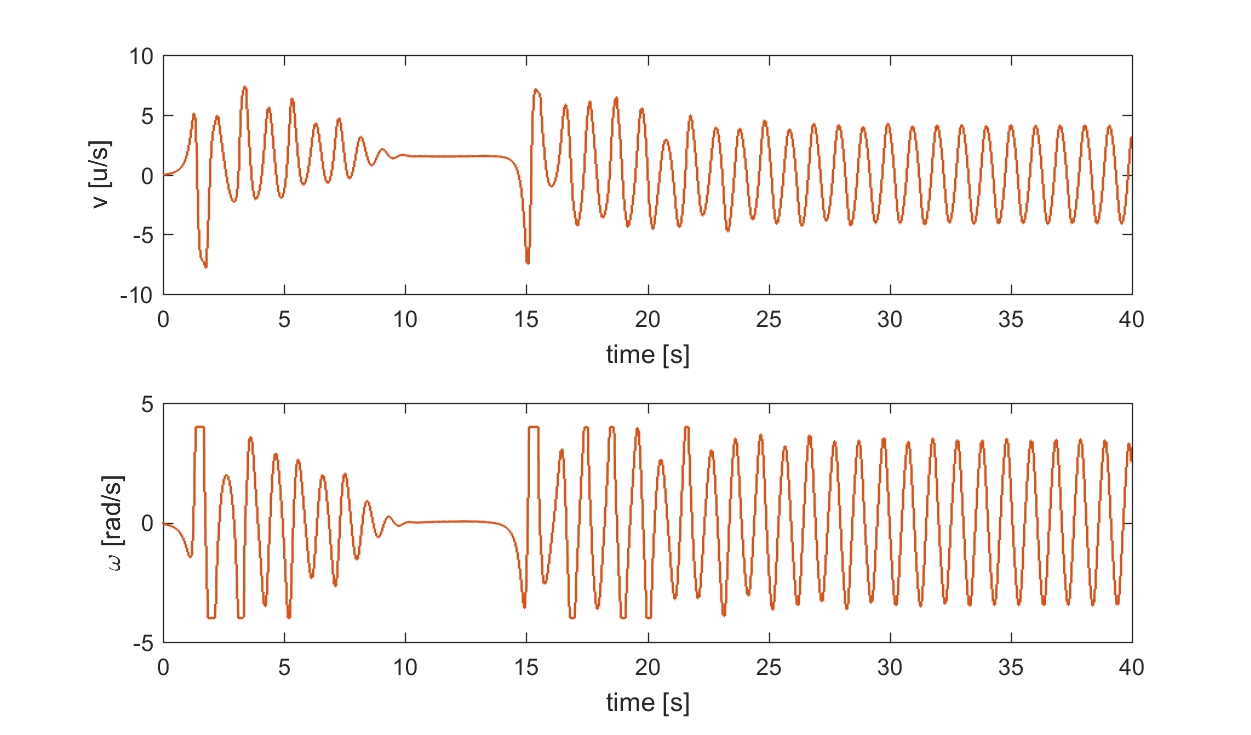
\includegraphics[width=1.4\textwidth]{nmpc_control.png}
\caption{\label{fig:nmpcu}Control action evolution.}
\end{subfigure}
\begin{subfigure}[t]{0.4\textwidth}
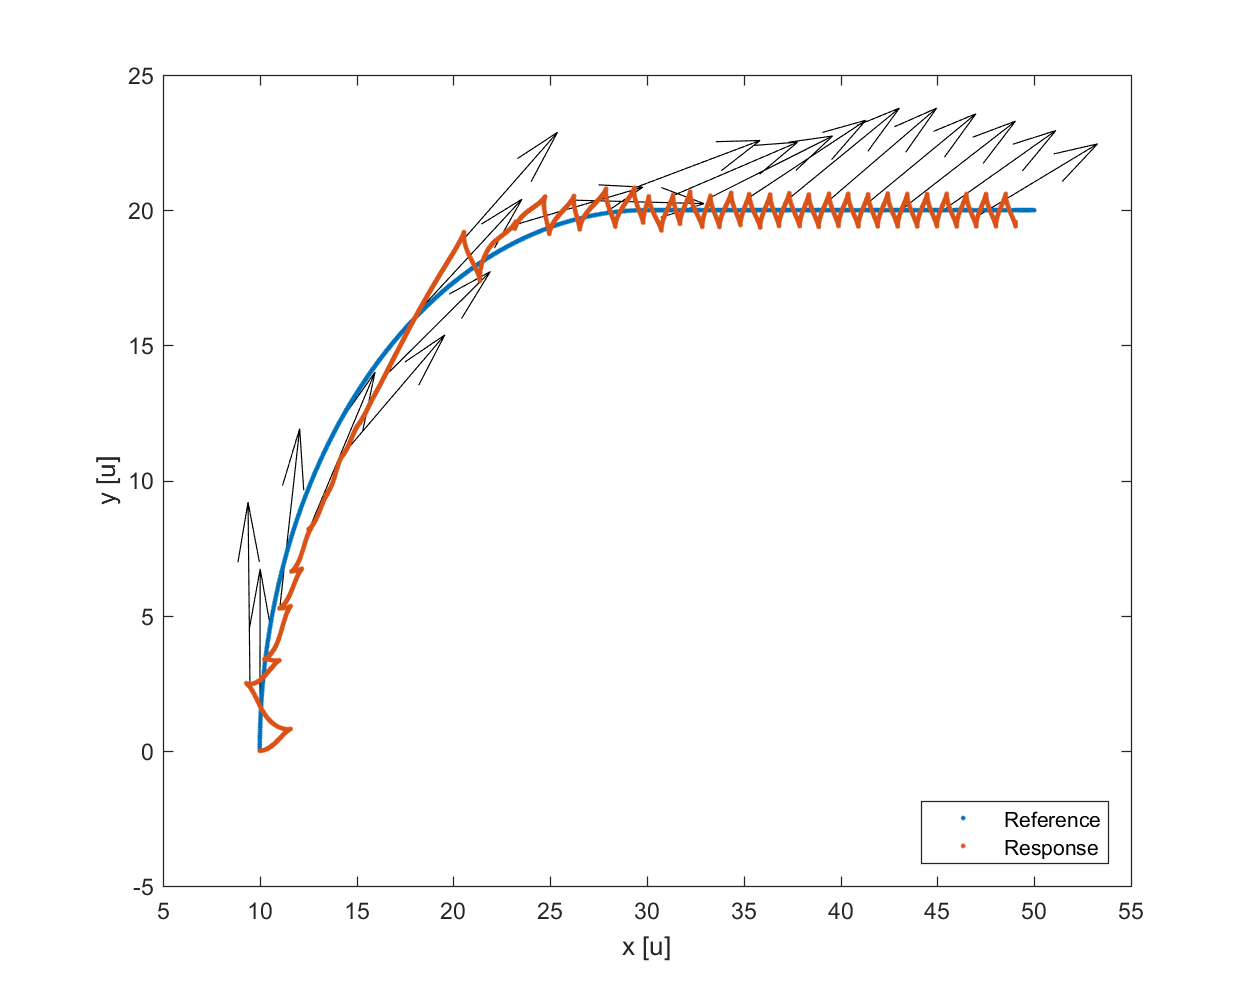
\includegraphics[width=1.4\textwidth]{nmpc_xy.png}
\caption{\label{fig:nmpcxy}Overall response of the system over the surface. Arrows at the given points correspond to orientation.}
\end{subfigure}
\caption{\label{fig:nmpc_simulation}NMPC Simulation: Compound of the obtained responses.}
\end{figure}

% \begin{figure}[H]
% \centering
% 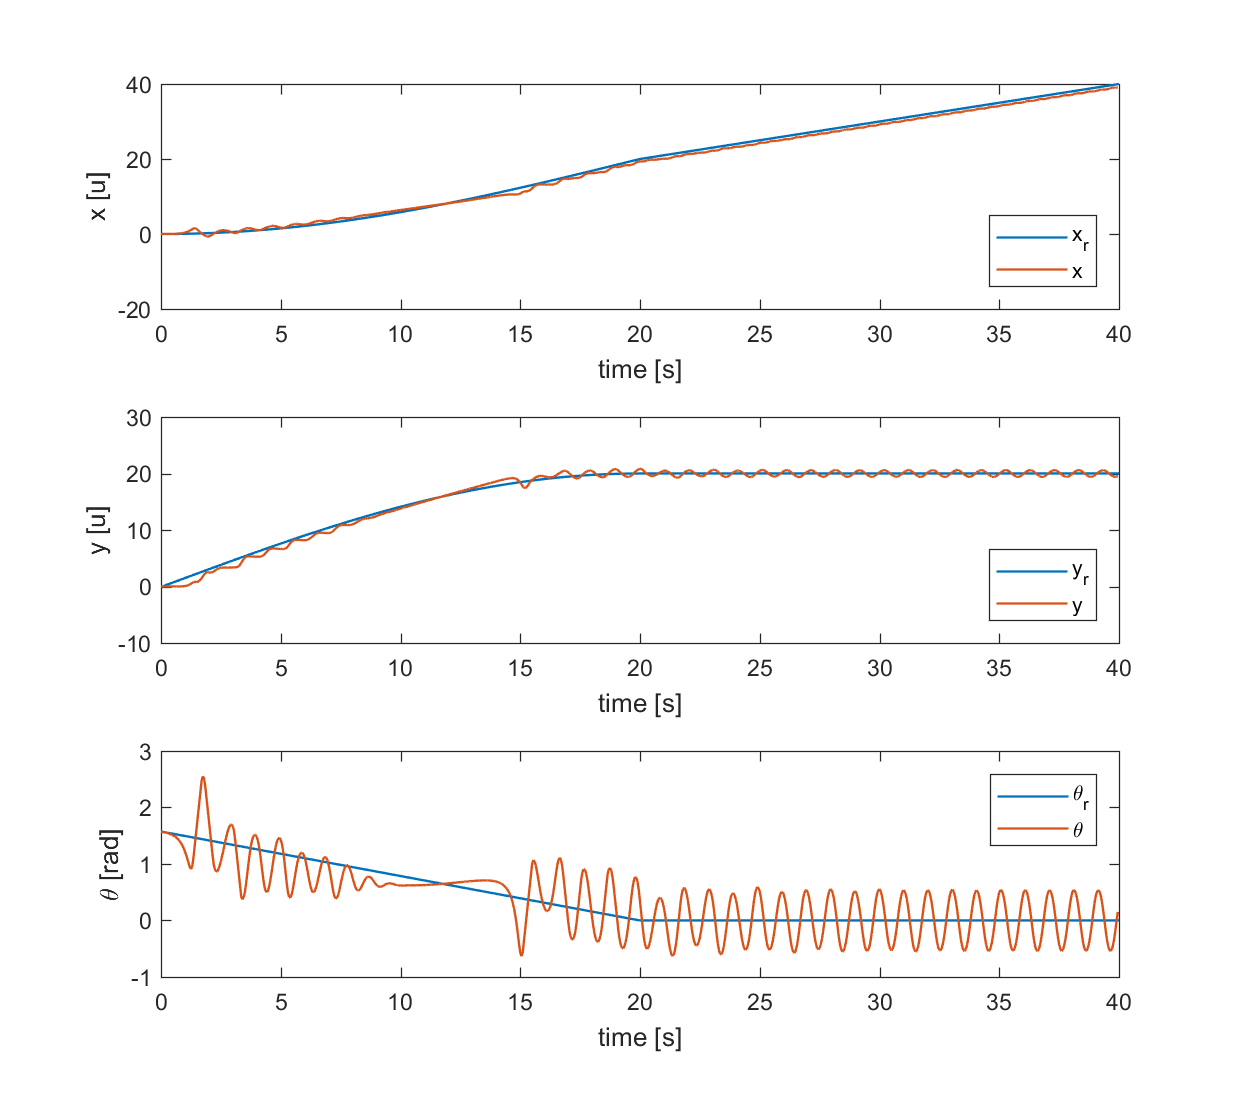
\includegraphics[width=0.5\textwidth]{nmpc_states.png}
% \caption{\label{fig:nmpcxl}NMPC Simulation: System's state behavior compared to its reference.}
% \end{figure}
% \begin{figure}[H]
% \centering
% 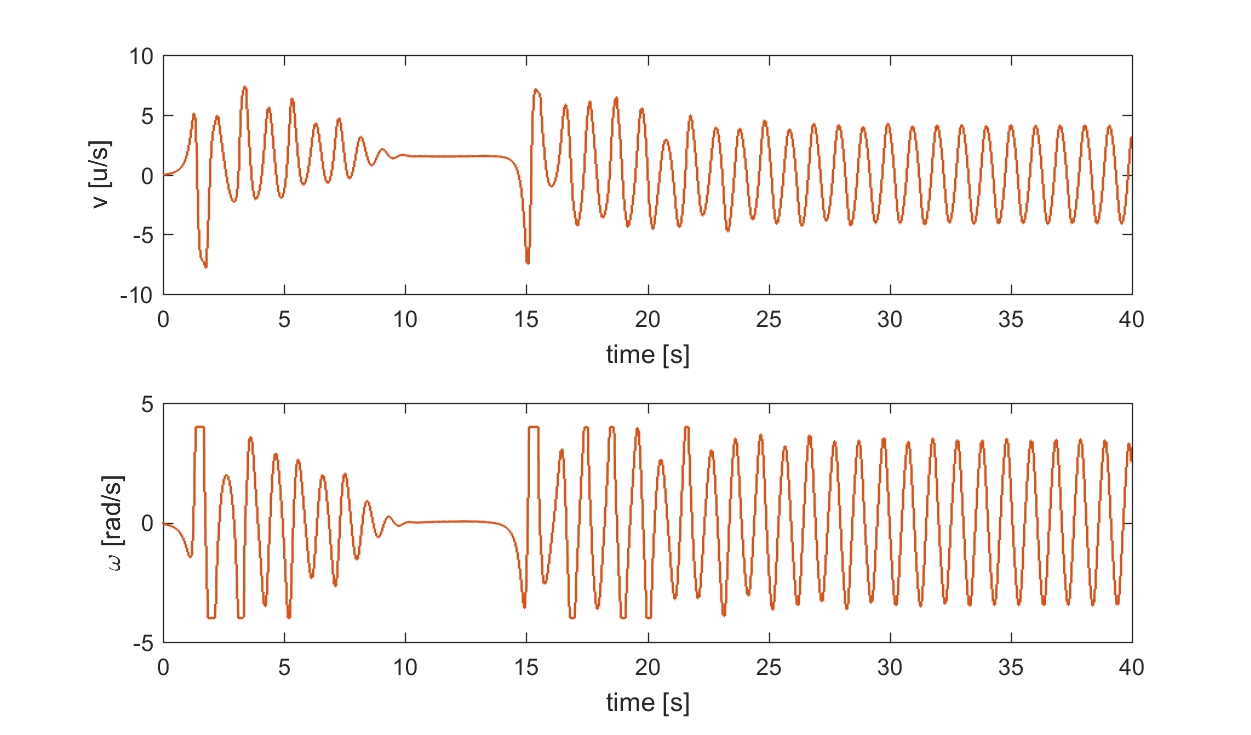
\includegraphics[width=0.5\textwidth]{nmpc_control.png}
% \caption{\label{fig:nmpcu}NMPC Simulation: Control action evolution.}
% \end{figure}
% \begin{figure}[H]
% \centering
% 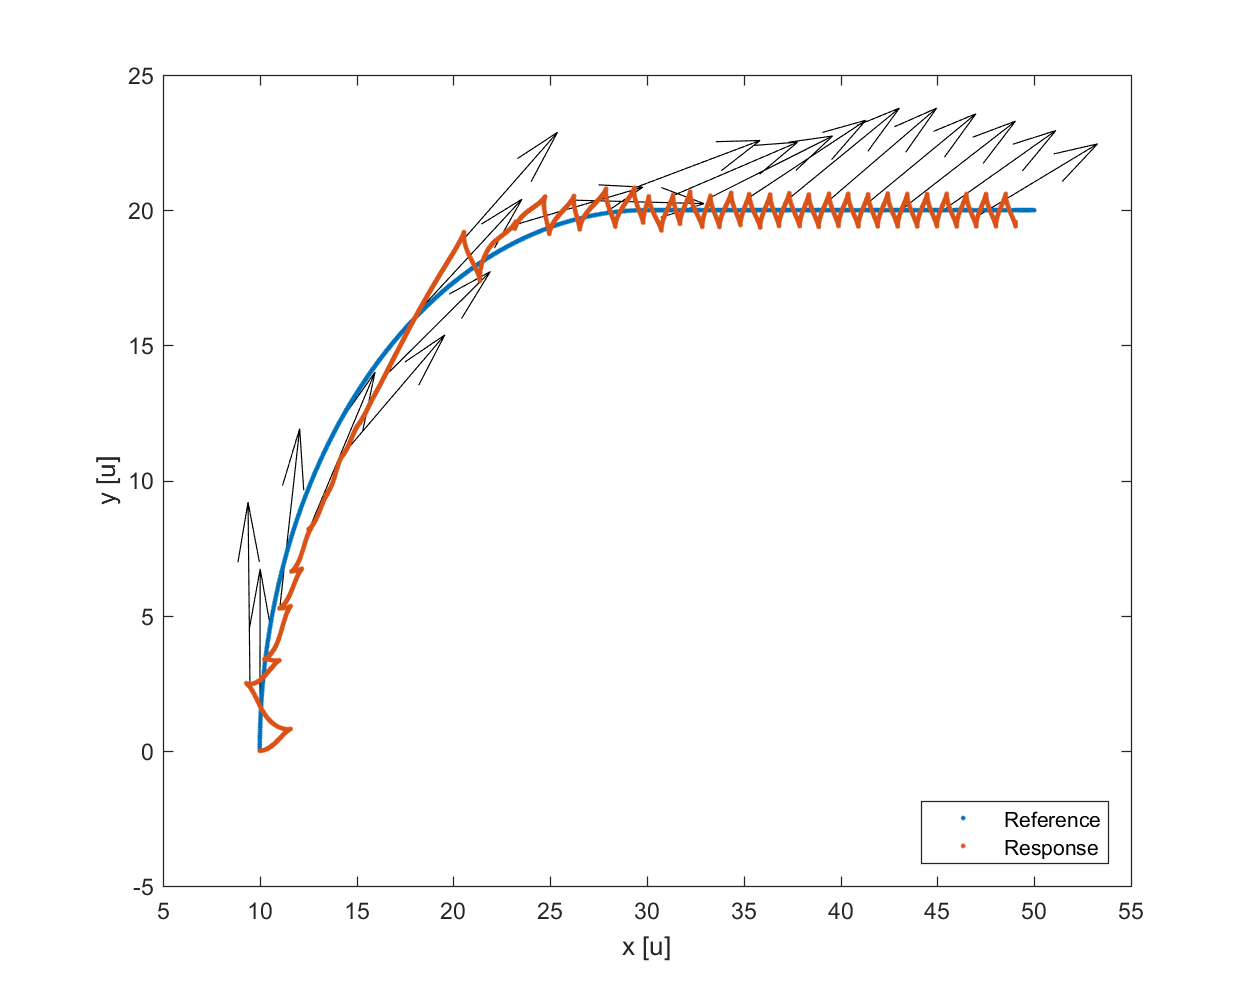
\includegraphics[width=0.5\textwidth]{nmpc_xy.png}
% \caption{\label{fig:nmpcxy}NMPC Simulation: Overall response of the system over the surface. Arrows at the given points correspond to orientation.}
% \end{figure}

\subsection{Results comparison}\label{CD}

For both methods we evaluate, as performance indexes, the 2-norm for the control actions and the states-reference error component independently. In table \ref{tab:index} their evaluation is shown. Main differences are the index for the \(\omega\) control action and the \(\theta\) state. Also the \(x\) states index shows great difference between the controllers.

The difference in the control action mainly happens because, while being both oscillating signals, the second controller produces a more smooth, hence slow, sequence which results in a greater energy consumption. The control action computed by the LMPC, while being more rough and chattering, is quicker, also producing more frequent but smaller errors. What is seen in the difference for the \(\theta\) state index.

For the same reason, the difference between the indexes for \(x\) state is produced. The LMPC is able to follow reliably the reference trajectory (with frequent errors but small), while the NMPC produce higher tracking error. We do not observe important differences between the indexes for \(y\) state, because in this case the LMPC accumulates a high error.

\begin{table}
\centering
\begin{tabular}{|c|c|c|c|}
	\hline
	Perf. Index & LMPC & NMPC \\
    \hline
    \hline
	\(\lVert v\rVert_{2}\) & \(201.11\) & \(261.41\) \\
    \(\lVert \omega\rVert_{2}\) & \(24.87\) & \(196.10\) \\
    \(\lVert e_x\rVert_{2}\) & \(9.75\) & \(77.61\) \\
    \(\lVert e_y\rVert_{2}\) & \(41.43\) & \(56.18\) \\
    \(\lVert e_{\theta}\rVert_{2}\) & \(1.24\) & \(37.03\) \\
    \hline
\end{tabular}
\caption{\label{tab:index}Performance indexes evaluation for both simulations.}
\end{table}


\subsection{Inverse Kinematics Module}\label{CE}

According to our control architecture (Fig. \ref{fig:control}), once the MPC obtains a control action, the inverse kinematics module, defined by Eq. \ref{eq:4} should obtain actuators position for the whole discretized surface. In order to check our kinematic definition, in Fig. \ref{fig:ikine} a computed result for a given instant control action is represented.

Notice that in order to only actuate over the needed actuators for a given reference, thus setting free the rest of the surface for other packages, and accounting on a delay for the actuators a state prediction for a future horizon would have to be implemented. If using MPC, its computed trajectory for the prediction horizon at each state could be used as an estimator.

\begin{figure}[H]
\centering
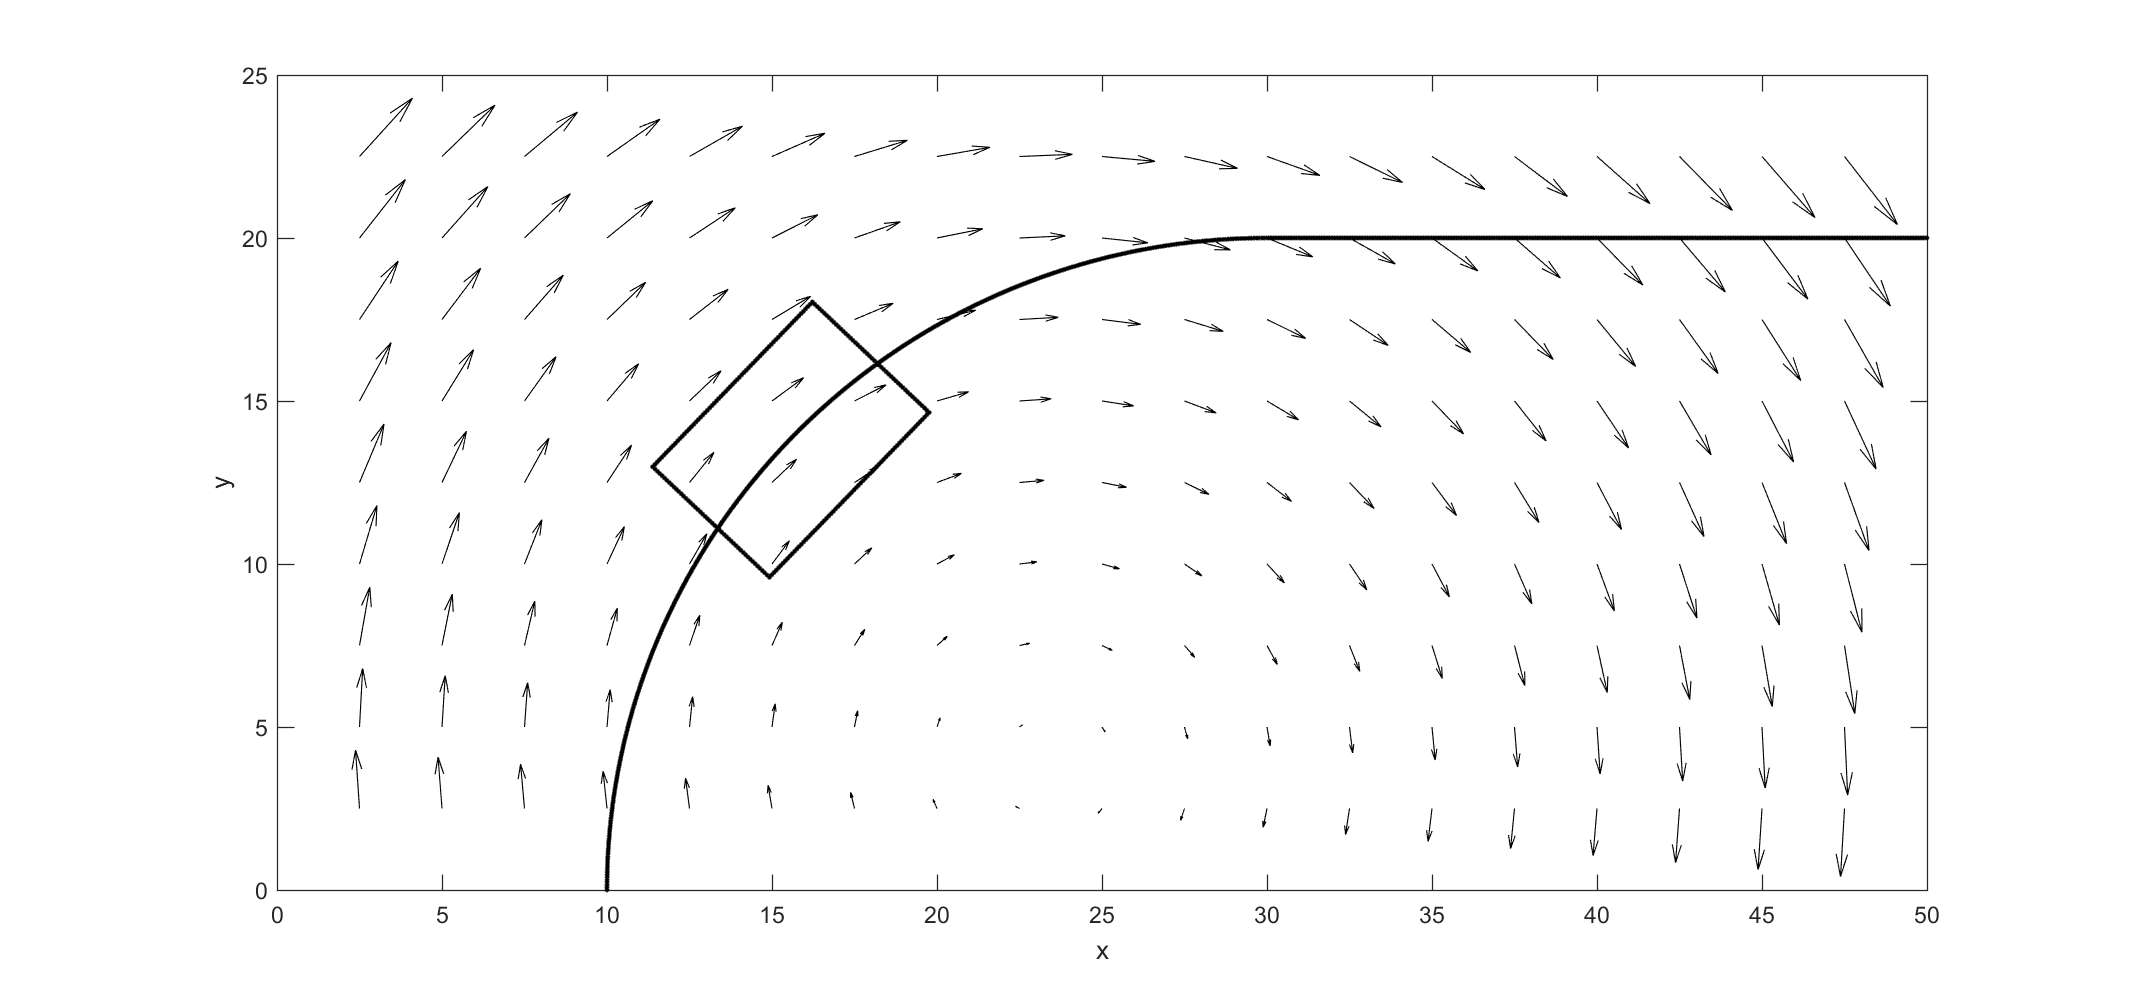
\includegraphics[width=0.5\textwidth]{ikine.png}
\caption{\label{fig:ikine}Example of the Inverse Kinematic module for a given instant. It computes the velocity vector that ensures the box, as a rigid body, draws the desired trajectory.}
\end{figure}


\section{Conclusions}

In this work a Model Based Predictive Control solution has been proposed and simulated for a Smart conveyor belt logistic system. The system modeled as a 2-DOF robot has been implemented to follow a plane trajectory.

The OCPs of the controllers considered, have been formulated optimizing reference error and control action 2-norms. This approach shows that does not prevent the control action from oscillating. A well-known improvement could be done, not weighting the control action 2-norm, but the variation of this. This has been proved that reduces control action oscillation, what at least is a result to be improved before a real implementation is considered.

Also, considering the dynamic model for the robot, as proposed in section I could produce better results. Despite these considerations, this scenario may not be the best case for a MPC. Other control architectures, also based in a dynamic model, such a classical manipulator controller with pre-computed torque feed-forward compensation could be studied.

\bibliographystyle{IEEEtran}
\bibliography{refs}

\end{document}